\chapter{Context}
\label{spec:ch:context}

This bachelor thesis is done by Simon Barras and supervised by Frederic Bapst and Jean Hennebert.
The customer Paolo Calafiura is a physicist and computer scientist at the \acrfull{lbl}.
To do this project, I am moving to Berkeley, California, for ten weeks.
The goal is to improve the performance of the project Celeritas, which is a particle physics simulation software accelerated by \acrshort{gpu}s.




\section{Celeritas}
\label{spec:ch:context:celeritas}

The project Celeritas~\cite{Celeritas-Project} is a particle physics simulation software that can be integrated with Geant4~\cite{geant4} as a plugin library.
It can also be used as a standalone application, with limited functionality for now.
Geant4 is a toolkit for the simulation of the path of particles through matter.
It is used for many detector simulation applications in particle physics, medical physics, and beyond.
The goal of the Celeritas project is to develop GPU-accelerated versions of the most computationally intensive kernels of Geant4.

\section{Physics simulation}
\label{spec:ch:context:physics-simulation}

Actually, the two main customers are \acrshort{cms} and \acrshort{atlas}, both made their experiments at the \acrfull{cern} with the \acrfull{lhc} and run their simulation with Geant4.
They are both using Geant4 and they didn't have committed to using Celeritas beyond an initial evaluation.
Detector simulation is used to validate and calibrate the algorithms used to estimate the properties of the primary particles from the observed detector data.
The main goal of the thesis will be to optimize a GPU-accelerated version of the Prince Dormand algorithm~\cite{princeDormand}, a Runge-Kutta solver~\cite{Runge-Kutta-methods} for the differential equations governing the trajectory of particles in a non-uniform magnetic field.
This work will improve the project Celeritas~\cite{Celeritas-Project} which may replace Geant4~\cite{geant4} in the future.

The \acrfull{atlas} experiment tracks the path of particles in the detector and produces coordinates points where particles traverse the sensors.
Figure \ref{spec:fig:context:physics-simulation:lhc} represents this experiment.
\begin{figure}[ht]
    \centering
    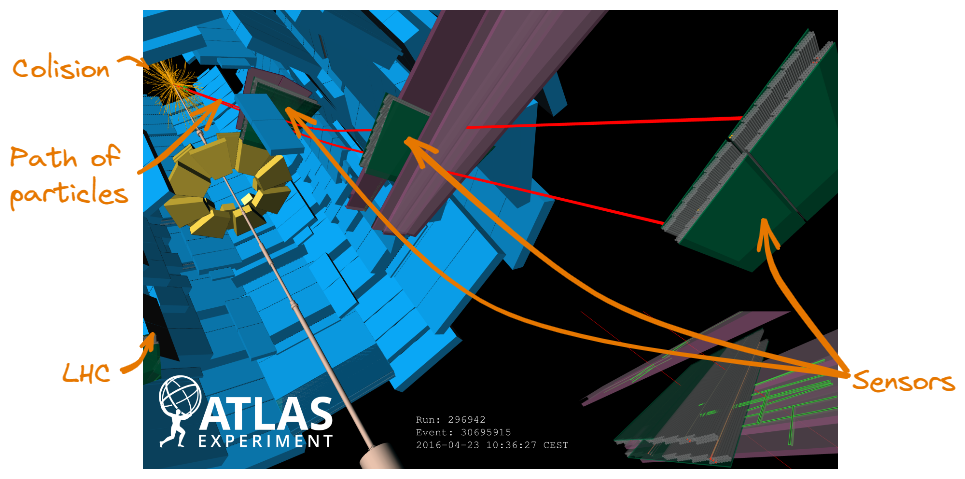
\includegraphics[width=0.85\textwidth]{05-resources/img/spec/experiment-atlas.excalidraw.png}
    \caption{ATLAS experiment at CERN~\cite{atlas-experiment}}
    \label{spec:fig:context:physics-simulation:lhc}
\end{figure}


\section{Lawrence Berkeley National Laboratory}
\label{spec:ch:context:lbl}

The \acrfull{lbl} is a national laboratory in Berkeley, California.
It is managed and operated by the University of California for the \acrfull{doe}.
The lab is situated in the hills of Berkeley and it is composed of many buildings and has a beautiful view of the San Francisco Bay (see Fig.\ref{spec:fig:context:lbl:lab-view}).

\begin{figure}[ht]
    \centering
    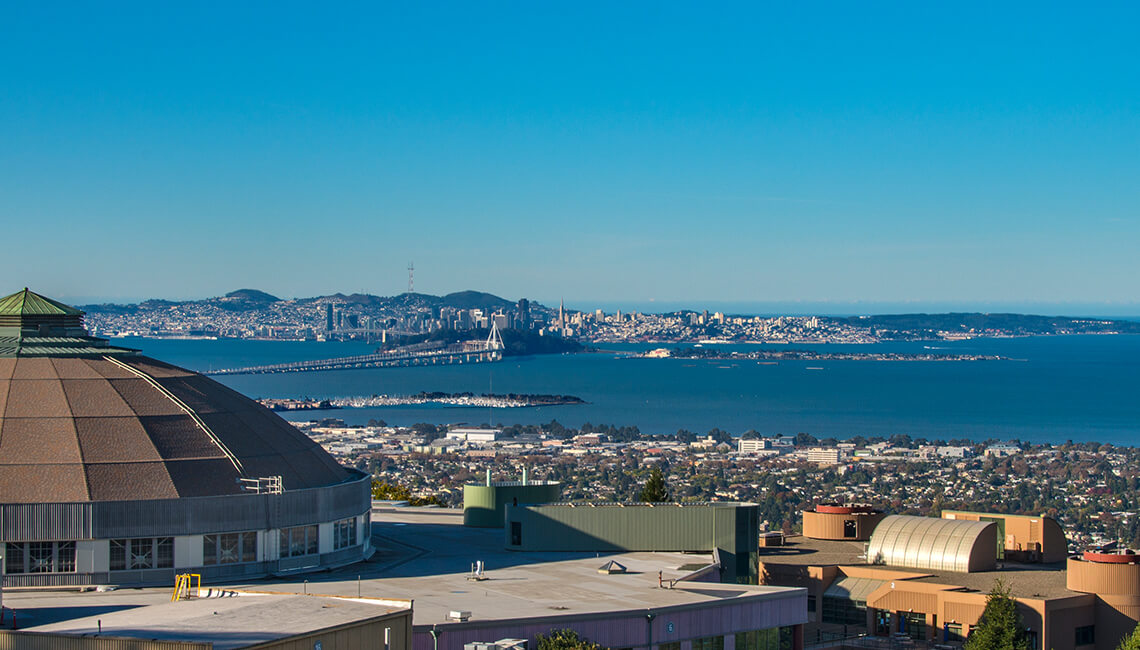
\includegraphics[width=0.8\textwidth]{05-resources/img/spec/lab-view.jpg}
    \caption{Lawrence Berkeley National Laboratory}
    \label{spec:fig:context:lbl:lab-view}
\end{figure}


The Physics and X-Ray Science Group, where the project is done, is situated in building 50f and the LBL ATLAS group, who are the customers of this project, are located in building 50.


\section{The Need}
\label{spec:ch:context:need}

Celeritas is already accelerated by \acrshort{gpu}s, however, the team wants to improve the performance to be able to reduce the time of a simulation.
In the current version of the code, each particle track is processed in parallel by one GPU thread, with no collaboration between threads.
GPU profiling of the code shows that execution time is dominated by two kernels.
The first one is handled by the interaction with the detector geometry to know where, in 3D space, the particle is situated and during the profiling, the library used is vecGeom~\cite{VecGeom}.
The second kernel, which will be the focus of this bachelor thesis project, is the computation of a differential equation using Dormand-Prince~\cite{princeDormand}.
